\chapter{التطبيق العملي: منظومة المقص الطائر (\textenglish{Flying Shear})}
\label{ch:practical_application}

% مقدمة الفصل
يُمثل هذا الفصل الجانب التطبيقي والعملي لمشروع مقرر "أتمتة 2"، حيث تُترجم النظريات الديناميكية إلى خوارزميات برمجية وتوصيلات فيزيائية. يُعالج هذا الفصل مسألة التحكم الدقيق في آلة "المقص الطائر" المستخدمة في خطوط إنتاج الصابون المستمرة. سيتم التدرج في بناء المنظومة بدءاً من الفهم الميكانيكي لحركة التطبيق، مروراً باختيار وتوزيع المداخل والمخارج على متحكم \textenglish{Delta DVP-28SV11T}، ثم استعراض المخطط الكهربائي لربط المشفرات ومحركات السيرفو، وصولاً إلى بناء خوارزمية التحكم بلغة المخطط السلمي (\textenglish{Ladder Logic}).

\vspace{0.5cm}

% استدعاء ملفات السكشنات بالترتيب
\section{نظرة عامة على المنظومة \textenglish{(Application Overview)}}
تُعد منظومة "المقص الطائر" \textenglish{(Flying Shear)} من التطبيقات الكلاسيكية والمتقدمة في آنٍ واحد داخل قطاع الأتمتة الصناعية، وتُستخدم بشكل واسع النطاق في خطوط الإنتاج المستمرة التي تعتمد على السحب أو التدفق المستمر، مثل خطوط إنتاج الصابون، الأنابيب البلاستيكية، والألواح المعدنية.

\subsection{المشكلة الصناعية والحل الهندسي}
في خطوط الإنتاج التقليدية، تتطلب عملية قص المنتج إيقاف السير الناقل تماماً لإجراء القطع، مما يؤدي إلى هدر كبير في الوقت، وانخفاض حاد في الإنتاجية، بالإضافة إلى احتمالية تراكم المواد أو تشوهها أثناء التوقف. من هنا برزت الحاجة لمنظومة "المقص الطائر"، والتي تكمن فكرتها الهندسية الأساسية في تحقيق \textbf{التزامن الحركي الكامل} \textenglish{(Kinematic Synchronization)}. 

حيث تتحرك عربة القص بشكل موازٍ للمنتج وبنفس سرعته الخطية تماماً، مما يجعل السرعة النسبية بينهما تساوي صفراً أثناء فترة القص. هذا التزامن يسمح بقطع المنتج أثناء حركته بدقة متناهية دون الحاجة إلى إيقاف خط الإنتاج، مما يرفع من كفاءة الآلة \textenglish{(OEE)} بشكل جذري.

\subsection{المكونات الأساسية للمنظومة المعمارية}
تتألف معمارية التحكم في هذه المنظومة من عدة محاور ميكانيكية وكهربائية تعمل بتناغم تام:
\begin{itemize}
    \item \textbf{المحور القائد \textenglish{(Master Axis)}:} وهو السير الناقل الذي يحمل شريط الصابون المستمر. يتم مراقبة سرعته وموقعه بدقة متناهية باستخدام مشفر دوراني نبضي \textenglish{(Rotary Encoder)} متصل ميكانيكياً بمحور السير.
    \item \textbf{المحور التابع \textenglish{(Slave Axis)}:} وهو عربة المقص التي تتحرك للأمام والخلف. يتم تحريكها بواسطة محرك سيرفو دقيق \textenglish{(Servo Motor)} قادر على تحقيق تسارع عالٍ واستجابة لحظية للأوامر.
    \item \textbf{العقل المدبر \textenglish{(Controller)}:} يُستخدم في هذا التطبيق متحكم منطقي مبرمج \textenglish{(PLC)} من عائلة \textenglish{Delta DVP}. يتميز هذا المتحكم بقدرته العالية على معالجة العدادات السريعة ذات الـ 32-بت \textenglish{(High-Speed Counters)} لقراءة نبضات المشفر، وقدرته على توليد نبضات عالية التردد \textenglish{(PTO)} للتحكم في درايف السيرفو.
    \item \textbf{آلية القص \textenglish{(Cutting Mechanism)}:} وتتمثل في أسطوانة هوائية \textenglish{(Pneumatic Cylinder)} مسؤولة عن إنزال ورفع شفرة القص في اللحظة التي يتحقق فيها التزامن الحركي التام.
\end{itemize}

\subsection{دورة عمل المنظومة \textenglish{(Operation Cycle)}}
تمر عربة المقص خلال دورة الإنتاج الواحدة بأربع مراحل فيزيائية أساسية، وهي التي سيتم بناء خوارزمية التحكم برمجياً على أساسها:
\begin{enumerate}
    \item \textbf{الانتظار \textenglish{(Standby)}:} وقوف العربة بوضع السكون عند نقطة الصفر بانتظار وصول طول المنتج للحد المطلوب.
    \item \textbf{التسارع والمزامنة \textenglish{(Acceleration \& Sync)}:} انطلاق العربة بتسارع عالٍ في أجزاء من الثانية حتى تتطابق سرعتها مع سرعة السير الناقل.
    \item \textbf{القص \textenglish{(Cutting)}:} تفعيل آلية القطع أثناء التطابق الحركي، مع إبقاء السكين للأسفل لفترة زمنية محددة لضمان اختراق المنتج.
    \item \textbf{العودة السريعة \textenglish{(Fast Return)}:} رفع الشفرة ورجوع العربة بأقصى سرعة ميكانيكية ممكنة إلى نقطة البداية لانتظار القطعة التالية.
\end{enumerate}

من خلال هذا التوصيف، يتضح أن التحدي الأكبر في هذه المنظومة ليس في عملية القطع بحد ذاتها، بل في \textbf{الخوارزمية البرمجية} القادرة على ربط المتغيرات الديناميكية (السرعة، المسافة، الزمن) ومعالجتها بالتوازي لضمان استقرار الآلة وجودة المنتج النهائي.
\section{توزيع المداخل والمخارج \textenglish{(I/O Mapping)}}
لضمان استقرار المنظومة وتجنب أي تعارض في البنية العتادية \textenglish{(Hardware Conflict)} للمتحكم، تمت دراسة وتوزيع المداخل والمخارج بدقة بناءً على المتطلبات الوظيفية للآلة ودليل الشركة المصنعة لمتحكمات دلتا \textenglish{(Delta DVP)}. يعتمد هذا التوزيع على تخصيص قنوات محددة للتعامل مع الإشارات عالية التردد (مثل نبضات المشفر ومخارج السيرفو)، مع ترك المداخل والمخارج العادية لمهام التحكم والحماية الكلاسيكية.

\subsection{الجدول الشامل للمداخل والمخارج}
يوضح الجدول التالي التوزيع المعتمد في هذه المنظومة لربط الحساسات والمشغلات مع منافذ المتحكم المنطقي:

\begin{table}[h!]
\centering
\renewcommand{\arraystretch}{1.5}
\begin{tabular}{|c|p{11cm}|}
\hline
\rowcolor{gray!20}
\textbf{العنوان} & \textbf{الوظيفة الميكانيكية والبرمجية} \\
\hline
\textbf{X0} & مفتاح بدء التشغيل وتفعيل النظام الميكانيكي \textenglish{(System Start)}. \\
\hline
\textbf{X1} & مفتاح الإيقاف العام للمنظومة \textenglish{(System Stop)}. \\
\hline
\textbf{X2} & إشارة الحماية من زيادة الحمل \textenglish{(Overload Protection)} لإيقاف النظام عند حدوث أخطاء كهربائية أو ميكانيكية. \\
\hline
\textbf{X3} & حساس المنتج الضوئي، ويُبرمج كحافة صاعدة \textenglish{(Rising Edge)} لتصفير العداد لمرة واحدة. \\
\hline
\textbf{X4} & قناة الطور الأول للمشفر \textenglish{(Phase A)} - مرتبطة عتادياً بالعداد السريع \textenglish{C254}. \\
\hline
\textbf{X5} & قناة الطور الثاني للمشفر \textenglish{(Phase B)} - مرتبطة عتادياً بالعداد السريع \textenglish{C254}. \\
\hline
\textbf{X6} & حساس نقطة الصفر \textenglish{(Home Sensor)} لإيقاف عربة المقص وتحديد نقطة الانطلاق. \\
\hline
\textbf{X7} & حساس نهاية الشوط الأمامي \textenglish{(Forward Limit Switch)} لعمل كبح طوارئ للمحرك. \\
\hline
\textbf{X10} & حساس نهاية الشوط الخلفي \textenglish{(Reverse Limit Switch)} لعمل كبح طوارئ للمحرك. \\
\hline
\textbf{Y0} & مخرج النبضات عالي التردد \textenglish{(Pulse Output)} للتحكم في سرعة ومسافة السيرفو. \\
\hline
\textbf{Y1} & مخرج تحديد الاتجاه \textenglish{(Direction)} لتمييز التقدم للأمام أو التراجع للخلف. \\
\hline
\textbf{Y2} & إشارة تفعيل محرك السيرفو والمحافظة على المغنطة \textenglish{(Servo Enable / SON)}. \\
\hline
\textbf{Y4} & مخرج تفعيل أسطوانة القص لإنزال السكين في لحظة التزامن. \\
\hline
\end{tabular}
\caption{\centering{توزيع المداخل والمخارج}}
\label{tab:io_mapping}
\end{table}

\section{التوصيل الفيزيائي والكهربائي مع الـ \textenglish{PLC}}
\label{sec:plc_wiring}

يتم توصيل جهاز الـ \textenglish{PLC} مع العتاد الخارجي بناءً على المواصفات الفنية للمتحكم \textenglish{DVP-28SV11T} وفق التوزيع الهندسي التالي:

\subsection{توصيل المشفر القائد (\textenglish{Master Encoder})}
يتم توصيل المشفر الدوار (الخاص بقراءة سرعة سير الصابون) بالمداخل السريعة \LR{(X4, X5)}. لتجنب التشويش، يُنصح بشدة باستخدام كابلات مجدولة ومحمية شيلد (\textenglish{Shielded Twisted Pair}) وتأريضها من طرف واحد فقط.
\begin{itemize}
    \item إشارة القناة (\textenglish{A}) تُوصل بالمدخل \LR{X4}.
    \item إشارة القناة (\textenglish{B}) تُوصل بالمدخل \LR{X5}.
    \item يُوصل الطرف المشترك (\textenglish{S/S}) بجهد $24\text{ VDC}$.
\end{itemize}

\subsection{توصيل مشغل السيرفو (\textenglish{Servo Drive})}
يتم التحكم بدرايف السيرفو عبر مخارج الترانزستور باستخدام بروتوكول (النبضة والاتجاه):
\begin{itemize}
    \item \textbf{إشارة النبضات (\textenglish{PULS}):} تُوصل بالمخرج السريع \LR{Y0} للتحكم بسرعة وموقع المقص.
    \item \textbf{إشارة الاتجاه (\textenglish{SIGN}):} تُوصل بالمخرج \LR{Y1} لتحديد اتجاه الدوران (أمام/خلف).
    \item \textbf{إشارة التفعيل (\textenglish{SON}):} تُوصل بالمخرج \LR{Y2} لتشغيل المحرك وتثبيته.
    \item \textbf{ملاحظة حماية:} تمت إضافة مقاومة $2.2\text{ k}\Omega$ على التوالي مع إشارات النبض والاتجاه لحماية الدوائر الداخلية لدرايف السيرفو.
\end{itemize}

\subsection{توصيل مفاتيح الحماية}
تُوصل إشارات السلامة (زر الإيقاف \LR{X1}، نهايات الشوط \LR{X7} و \LR{X10}، وإشارة الحماية الحرارية \LR{X2}) باستخدام تلامسات مغلقة طبيعياً \LR{(NC)}. يضمن ذلك إيقاف النظام الأوتوماتيكي فوراً في حالة الخطر أو عند انقطاع أي سلك بالخطأ.
ويبين الشكل \ref{fig:full_wiring_diagram} عملية توصيل المنظومة 
\\

\begin{figure}[h!]
    \centering
    \resizebox{\textwidth}{!}{%
    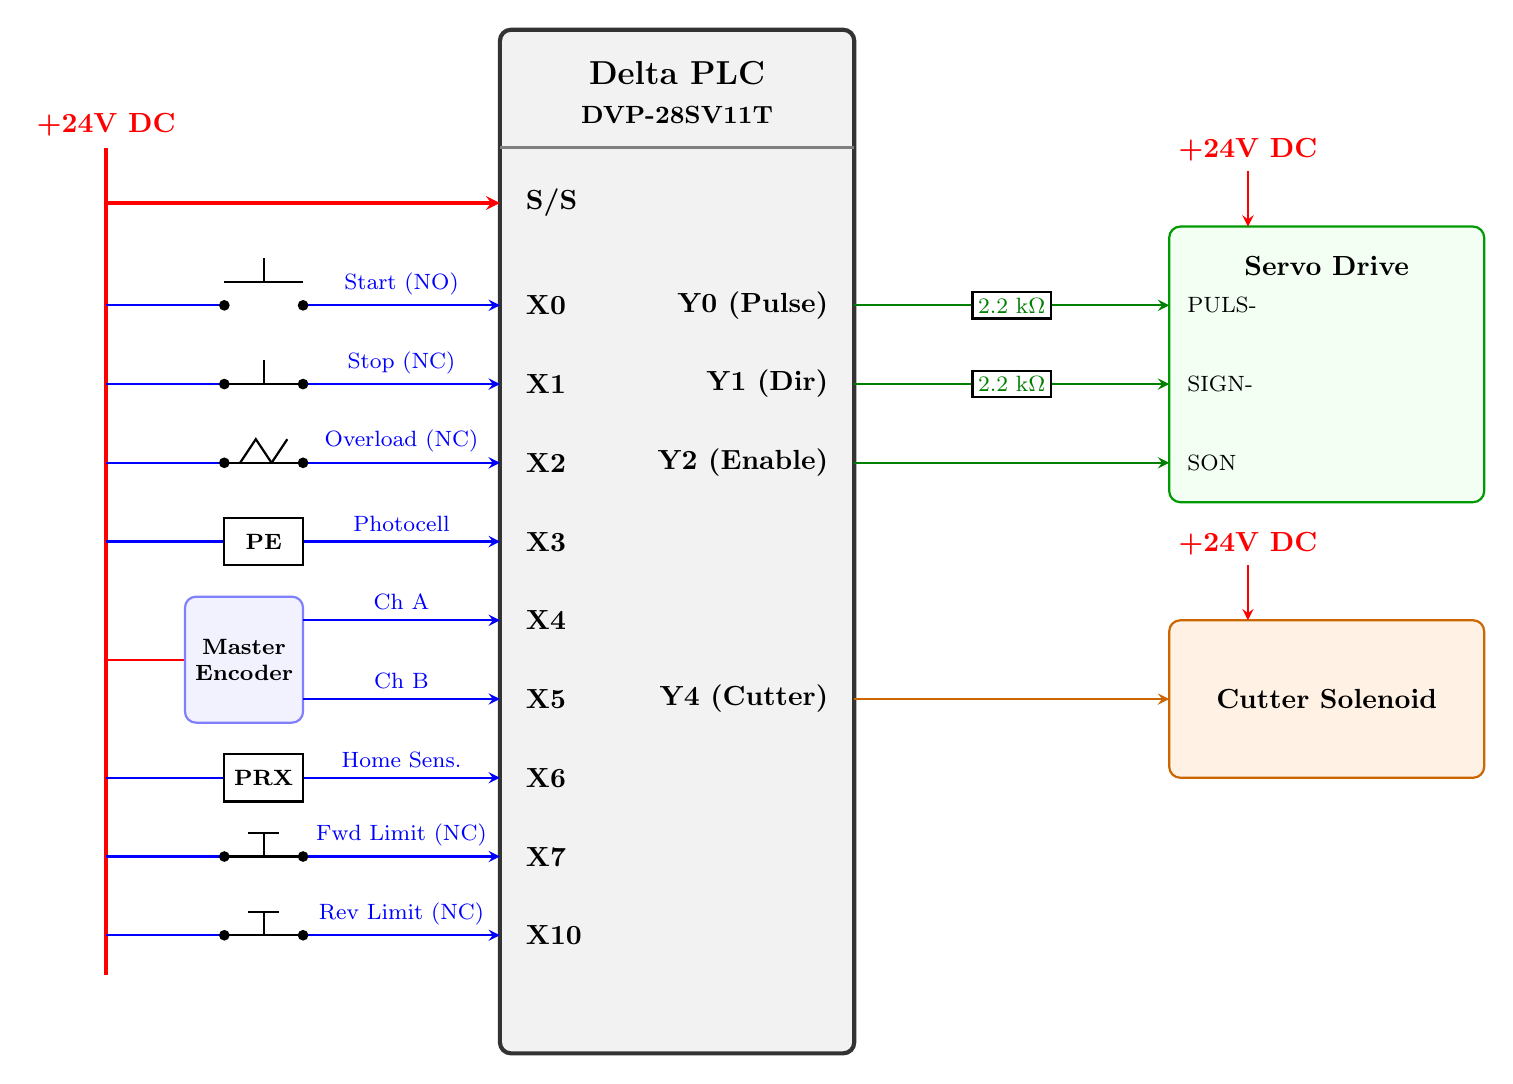
\begin{tikzpicture}[>=stealth, thick, text=black]

    % ==========================================
    % 1. PLC BLOCK
    % ==========================================
    \draw[fill=gray!10, draw=black!80, line width=1.5pt, rounded corners] (5, 0) rectangle (9.5, 13);
    \node[align=center, font=\large\bfseries] at (7.25, 12.2) {Delta PLC \\ \small DVP-28SV11T};
    \draw[line width=1pt, black!50] (5, 11.5) -- (9.5, 11.5);

    % Common 24V Line for Inputs
    \draw[red, line width=1.5pt] (0, 1) -- (0, 11.5) node[above, font=\bfseries] {+24V DC};

    % S/S Terminal
    \node[anchor=west, font=\bfseries] at (5.2, 10.8) {S/S};
    \draw[red, line width=1.2pt, ->] (0, 10.8) -- (5, 10.8);

    % Input Labels Inside PLC
    \foreach \y/\label in {9.5/X0, 8.5/X1, 7.5/X2, 6.5/X3, 5.5/X4, 4.5/X5, 3.5/X6, 2.5/X7, 1.5/X10} {
        \node[anchor=west, font=\bfseries] at (5.2, \y) {\label};
    }

    % ==========================================
    % 2. INPUTS (Drawing Electrical Symbols)
    % ==========================================

    % X0: Start (NO Pushbutton)
    \draw[blue, thick] (0, 9.5) -- (1.5, 9.5);
    \draw[blue, thick, ->] (2.5, 9.5) -- (5, 9.5) node[midway, above, font=\footnotesize] {Start (NO)};
    \filldraw[black] (1.5, 9.5) circle (1.5pt);
    \filldraw[black] (2.5, 9.5) circle (1.5pt);
    \draw[black, thick] (1.5, 9.8) -- (2.5, 9.8); % NO bridge
    \draw[black, thick] (2.0, 9.8) -- (2.0, 10.1); % Plunger

    % X1: Stop (NC Pushbutton)
    \draw[blue, thick] (0, 8.5) -- (1.5, 8.5);
    \draw[blue, thick, ->] (2.5, 8.5) -- (5, 8.5) node[midway, above, font=\footnotesize] {Stop (NC)};
    \filldraw[black] (1.5, 8.5) circle (1.5pt);
    \filldraw[black] (2.5, 8.5) circle (1.5pt);
    \draw[black, thick] (1.5, 8.5) -- (2.5, 8.5); % NC touching
    \draw[black, thick] (2.0, 8.5) -- (2.0, 8.8); % Plunger

    % X2: Thermal Overload (NC)
    \draw[blue, thick] (0, 7.5) -- (1.5, 7.5);
    \draw[blue, thick, ->] (2.5, 7.5) -- (5, 7.5) node[midway, above, font=\footnotesize] {Overload (NC)};
    \filldraw[black] (1.5, 7.5) circle (1.5pt);
    \filldraw[black] (2.5, 7.5) circle (1.5pt);
    \draw[black, thick] (1.5, 7.5) -- (2.5, 7.5); % NC touching
    \draw[black, thick] (1.7, 7.5) -- (1.9, 7.8) -- (2.1, 7.5); % Thermal zigzag symbol
    \draw[black, thick] (2.1, 7.5) -- (2.3, 7.8);

    % X3: Photocell (Sensor Box)
    \draw[blue, thick] (0, 6.5) -- (1.5, 6.5);
    \draw[blue, thick, ->] (2.5, 6.5) -- (5, 6.5) node[midway, above, font=\footnotesize] {Photocell};
    \draw[fill=white, draw=black, thick] (1.5, 6.2) rectangle (2.5, 6.8);
    \node[font=\footnotesize\bfseries] at (2.0, 6.5) {PE};

    % X4, X5: Master Encoder
    \draw[red, thick] (0, 5.0) -- (1.0, 5.0);
    \draw[fill=blue!5, draw=blue!50, thick, rounded corners] (1.0, 4.2) rectangle (2.5, 5.8);
    \node[align=center, font=\footnotesize\bfseries] at (1.75, 5.0) {Master\\Encoder};
    \draw[blue, thick, ->] (2.5, 5.5) -- (5, 5.5) node[midway, above, font=\footnotesize] {Ch A};
    \draw[blue, thick, ->] (2.5, 4.5) -- (5, 4.5) node[midway, above, font=\footnotesize] {Ch B};

    % X6: Home Sensor (Proximity)
    \draw[blue, thick] (0, 3.5) -- (1.5, 3.5);
    \draw[blue, thick, ->] (2.5, 3.5) -- (5, 3.5) node[midway, above, font=\footnotesize] {Home Sens.};
    \draw[fill=white, draw=black, thick] (1.5, 3.2) rectangle (2.5, 3.8);
    \node[font=\footnotesize\bfseries] at (2.0, 3.5) {PRX};

    % X7: Forward Limit (NC Switch)
    \draw[blue, thick] (0, 2.5) -- (1.5, 2.5);
    \draw[blue, thick, ->] (2.5, 2.5) -- (5, 2.5) node[midway, above, font=\footnotesize] {Fwd Limit (NC)};
    \filldraw[black] (1.5, 2.5) circle (1.5pt);
    \filldraw[black] (2.5, 2.5) circle (1.5pt);
    \draw[black, thick] (1.5, 2.5) -- (2.5, 2.5); % NC touching
    \draw[black, thick] (2.0, 2.5) -- (2.0, 2.8);
    \draw[black, thick] (1.8, 2.8) -- (2.2, 2.8); % Roller T-shape

    % X10: Reverse Limit (NC Switch)
    \draw[blue, thick] (0, 1.5) -- (1.5, 1.5);
    \draw[blue, thick, ->] (2.5, 1.5) -- (5, 1.5) node[midway, above, font=\footnotesize] {Rev Limit (NC)};
    \filldraw[black] (1.5, 1.5) circle (1.5pt);
    \filldraw[black] (2.5, 1.5) circle (1.5pt);
    \draw[black, thick] (1.5, 1.5) -- (2.5, 1.5); % NC touching
    \draw[black, thick] (2.0, 1.5) -- (2.0, 1.8);
    \draw[black, thick] (1.8, 1.8) -- (2.2, 1.8); % Roller T-shape

    % ==========================================
    % 3. OUTPUTS
    % ==========================================

    % Output Labels Inside PLC
    \foreach \y/\label in {9.5/Y0 (Pulse), 8.5/Y1 (Dir), 7.5/Y2 (Enable), 4.5/Y4 (Cutter)} {
        \node[anchor=east, font=\bfseries] at (9.3, \y) {\label};
    }

    % Servo Drive Box
    \draw[fill=green!5, draw=green!60!black, rounded corners, thick] (13.5, 7) rectangle (17.5, 10.5);
    \node[align=center, font=\bfseries] at (15.5, 10.0) {Servo Drive};
    
    % Servo Drive Terminals Text
    \node[anchor=west, font=\footnotesize] at (13.6, 9.5) {PULS-};
    \node[anchor=west, font=\footnotesize] at (13.6, 8.5) {SIGN-};
    \node[anchor=west, font=\footnotesize] at (13.6, 7.5) {SON};

    % Servo Wiring with Resistors
    \draw[green!50!black, thick, ->] (9.5, 9.5) -- (13.5, 9.5) node[midway, fill=white, draw=black, inner sep=2pt, font=\footnotesize] {2.2 k$\Omega$};
    \draw[green!50!black, thick, ->] (9.5, 8.5) -- (13.5, 8.5) node[midway, fill=white, draw=black, inner sep=2pt, font=\footnotesize] {2.2 k$\Omega$};
    \draw[green!50!black, thick, ->] (9.5, 7.5) -- (13.5, 7.5);
    
    % Servo +24V Supply
    \draw[red, thick, <-] (14.5, 10.5) -- (14.5, 11.2) node[above, font=\bfseries] {+24V DC};
    
    % Cutter Solenoid Box
    \draw[fill=orange!10, draw=orange!80!black, rounded corners, thick] (13.5, 3.5) rectangle (17.5, 5.5);
    \node[align=center, font=\bfseries] at (15.5, 4.5) {Cutter Solenoid};
    
    % Cutter Wiring
    \draw[orange!80!black, thick, ->] (9.5, 4.5) -- (13.5, 4.5);
    
    % Cutter +24V Supply
    \draw[red, thick, <-] (14.5, 5.5) -- (14.5, 6.2) node[above, font=\bfseries] {+24V DC};

    \end{tikzpicture}
    }
    \caption[المخطط الشامل لتوصيل المداخل والمخارج]{\centering المخطط الشامل لتوصيل المداخل والمخارج مع جهاز الـ \textenglish{PLC} لمنظومة المقص الطائر.}
    \label{fig:full_wiring_diagram}
\end{figure}
\section{الحسابات الديناميكية وضبط المعايير \textenglish{(Kinematics \& Parameterization)}}
\label{sec:kinematics_and_parameters}

يُعد هذا المبحث العصب الرياضي لمنظومة المقص الطائر، حيث يتم تحويل المتطلبات الإنتاجية (سرعة السير وطول المنتج) إلى قيم نبضية وترددات رقمية يتعامل معها جهاز الـ \textenglish{PLC}. تعتمد الحسابات على تحقيق التزامن التام بين المحور القائد (المشفر) والمحور التابع (محرك السيرفو).

\subsection{حسابات المحور القائد \textenglish{(Master Axis - Encoder)}}
يعتمد النظام على قراءة سرعة وموقع سير الصابون عبر المشفر النبضي لتحديد لحظة القص.
\begin{itemize}
    \item \textbf{دقة المشفر الميكانيكية:} تمت معايرة المشفر بحيث يُعطي $1000\text{ pulses}$ (نبضة) لكل مسافة مقطوعة قدرها $100\text{ mm}$ من حركة السير الناقل.
    \item \textbf{الطول المطلوب للمنتج:} $20\text{ cm}$ وهو ما يعادل $200\text{ mm}$.
    \item \textbf{حساب نبضات القص:} لمعرفة القيمة التي يجب أن يصل إليها العداد السريع (\textenglish{C254}) لاتخاذ قرار القص، نستخدم التناسب الخطي:
    $$x = \frac{200\text{ mm} \times 1000\text{ pulses}}{100\text{ mm}} = 2000\text{ pulses}$$
    إذن، الشرط البرمجي لتفعيل عملية القص هو وصول العداد إلى $2000$ نبضة.
\end{itemize}

\subsection{حسابات المحور التابع \textenglish{(Slave Axis - Servo Motor)}}
يُستخدم محرك سيرفو من طراز \textenglish{ASDA-B2} باستطاعة $400\text{ W}$ لتحريك عربة المقص.
\begin{itemize}
    \item \textbf{دقة المحرك الافتراضية:} يحتاج المحرك إلى $10,000\text{ pulses}$ لإتمام دورة ميكانيكية كاملة (\textenglish{1 Rev}).
    \item \textbf{الخطوة الميكانيكية (\textenglish{Pitch/Lead}):} كل دورة كاملة للمحرك تُحرك العربة مسافة $10\text{ mm}$.
    \item \textbf{النبضات لكل مليمتر:} 
    $$\text{Pulses per mm} = \frac{10,000\text{ pulses}}{10\text{ mm}} = 1000\text{ pulses/mm}$$
\end{itemize}

\subsection{سرعة التزامن والتردد المطلوب}
لتحقيق التزامن الحركي التام أثناء القص، يجب أن تكون السرعة الخطية لعربة المقص مساوية تماماً للسرعة الخطية لسير الصابون، والتي تبلغ في هذه المنظومة $\mathbf{150\text{ mm/s}}$.
\begin{itemize}
    \item \textbf{حساب تردد المزامنة:} لمعرفة التردد النبضي الذي يجب أن يرسله الـ \textenglish{PLC} للمحرك لكي ينطلق بهذه السرعة، نقوم بضرب السرعة الخطية في عدد النبضات اللازمة لقطع مليمتر واحد:
    $$f = v \times \text{Pulses per mm} = 150\text{ mm/s} \times 1000\text{ pulses/mm} = 150,000\text{ Hz}$$
\end{itemize}

التردد الناتج ($150\text{ kHz}$) يقع ضمن النطاق التشغيلي الآمن لمخارج الترانزستور في متحكم \textenglish{Delta DVP-28SV11T} (والذي يدعم حتى $200\text{ kHz}$). بناءً على ذلك، تم اعتماد هذا التردد في تعليمة توليد النبضات (\LR{DPLSY}) لضمان انطلاق السيرفو بسرعة التطابق المطلوبة بشكل سلس ومستقر.

\subsection{التحليل الهندسي لترددات التشغيل \textenglish{(Operating Frequencies Analysis)}}
يعكس هذا التصميم توازناً هندسياً دقيقاً ومدروساً بين متطلبات القراءة (المداخل) ومتطلبات الحركة (المخارج) في جهاز الـ \textenglish{PLC}، حيث تم تجنب رفع الترددات بشكل عشوائي:

\begin{itemize}
    \item \textbf{تردد القراءة الآمن (المحور القائد):} بضبط دقة المشفر على $10\text{ pulses/mm}$ (أي $1000$ نبضة لكل $100\text{ mm}$) وسرعة السير $150\text{ mm/s}$، فإن التردد الداخل للعداد السريع يبلغ $1500\text{ Hz}$ ($1.5\text{ kHz}$) فقط. هذا التردد المنخفض نسبياً يضمن استقراراً عالياً في القراءة ومناعة ممتازة ضد التشويش الكهرومغناطيسي \textenglish{(EMI)} في البيئة الصناعية، مع الاحتفاظ بدقة قياس ممتازة للتطبيق ($0.1\text{ mm}$).
    
    \item \textbf{تردد التحكم الدقيق (المحور التابع):} على الجانب الآخر، ولضمان أقصى درجات النعومة والدقة في حركة السيرفو أثناء القص، تم إبقاء دقة المحرك عالية جداً عند $1000\text{ pulses/mm}$. لتحقيق سرعة المزامنة ($150\text{ mm/s}$)، يقوم الـ \textenglish{PLC} بتوليد نبضات بتردد $150,000\text{ Hz}$ ($150\text{ kHz}$).
\end{itemize}

تُثبت هذه الأرقام كفاءة توظيف متحكم \textenglish{Delta DVP-28SV11T}، والذي استطاع الربط بين إشارة قراءة منخفضة ومستقرة من جهة، وتوليد إشارة تحكم سريعة وعالية الدقة من جهة أخرى، وكلاهما يعملان بشكل متزامن وبأمان تام تحت سقف القدرة العتادية القصوى للمنافذ ($200\text{ kHz}$).
\clearpage


\section{بناء الخوارزمية البرمجية \textenglish{(Ladder Logic Implementation)}}
\label{sec:ladder_code}

يُمثل المخطط السلمي \textenglish{(Ladder Diagram)} العقل المدبر للمنظومة، حيث تمت كتابة الخوارزمية باستخدام بيئة التطوير \textenglish{WPLSoft}. تم تصميم الكود ليتعامل مع متغيرات ديناميكية سريعة جداً، مما استدعى استخدام تعليمات متقدمة بحجم 32-بت \textenglish{(Double Word)} لضمان عدم حدوث أي تجاوز لسعة المسجلات \textenglish{(Overflow)} أثناء قراءة المشفر أو إرسال النبضات.

الشكل (\ref{fig:ladder_code}) يوضح المخطط السلمي الكامل للمنظومة كما تم تصديره من بيئة التطوير.


\subsection{التحليل الهندسي لبنية الكود}
ينقسم الكود البرمجي إلى أربع كتل وظيفية رئيسية، تم تصميم كل منها لمعالجة تحدٍ ديناميكي محدد في الآلة:

\subsubsection{1. العداد السريع والتصفير الذاتي \textenglish{(High-Speed Counter \& Self-Reset)}}
تم استخدام التعليمة \LR{DCNT C254 K0} لتفعيل قراءة نبضات المشفر القائد. القيمة \LR{K0} هنا مقصودة هندسياً؛ حيث تُوجه المتحكم لتجاهل أي هدف للعداد وجعله يعمل كـ "مسجل موقع مستمر". 
ولضمان عدم تراكم الخطأ أو ضياع مسافة أثناء عملية القص، تم ابتكار حيلة "التصفير الذاتي". بدلاً من انتظار انتهاء دورة القص لتصفير العداد، يتم أخذ نبضة حافة صاعدة \textenglish{(Rising Edge)} من ماركر المزامنة \LR{M2} لتصفير العداد \LR{C254} في اللحظة الأولى لبدء القطع، مما يضمن دقة متناهية للقطعة التالية حتى وإن كان المنتج مستمراً بالحركة.

\subsubsection{2. اتخاذ قرار القص \textenglish{(Cutting Decision)}}
نظراً لأن العداد \LR{C254} هو مسجل 32-بت، تم استخدام تعليمة المقارنة المزدوجة \LR{DLD>= C254 K2000}. هذا السطر يراقب القيمة المتراكمة باستمرار، وبمجرد وصولها إلى 2000 (والتي تكافئ طول الصابون المطلوب 20 سم)، يتم تفعيل حالة الانطلاق والمزامنة \LR{M2} بشكل فوري.

\subsubsection{3. توليد النبضات والتزامن \textenglish{(Pulse Output \& Synchronization)}}
لتحقيق التطابق الحركي مع السير الناقل، تم إرسال نبضات عالية التردد لدرايف السيرفو باستخدام التعليمة \LR{DPLSY K150000 K0 Y0}. 
التردد 150,000 هرتز تم حسابه بدقة بناءً على سرعة المنتج (150مم/ثانية) والنسبة الإلكترونية المعدلة في السيرفو (500 نبضة/مم). أما القيمة \LR{K0} في المسافة، فتعني إبقاء توليد النبضات مستمراً لضمان بقاء المقص متزامناً تماماً مع المنتج طوال فترة نزول الشفرة، على أن يتم الإيقاف لاحقاً عبر المؤقتات الزمنية.

\subsubsection{4. شبكات الحماية الميكانيكية \textenglish{(Protection Networks)}}
تم وضع تماسات حساسات نهاية الشوط \LR{X7} و \LR{X10} في نهاية الكود كشبكات حماية مستقلة. في حال تجاوز العربة لمسارها المسموح، تقوم هذه التماسات بعمل \textenglish{Reset} لحالات الحركة (\LR{M1, M2, M3}) مما يقطع النبضات عن التعليمة \LR{DPLSY} فوراً. هذه الطريقة البرمجية توقف الحركة مع إبقاء المحرك ممغنطاً \textenglish{(Servo Hold)} لمنع اندفاع العربة بسبب القصور الذاتي، وهو إجراء أأمن بكثير من قطع إشارة التفعيل \LR{Y2} بشكل مباشر.

\begin{figure}[h!]
    \centering
    % تأكد من أن مسار المجلد resources صحيح ومطابق لما لديك في المشروع
    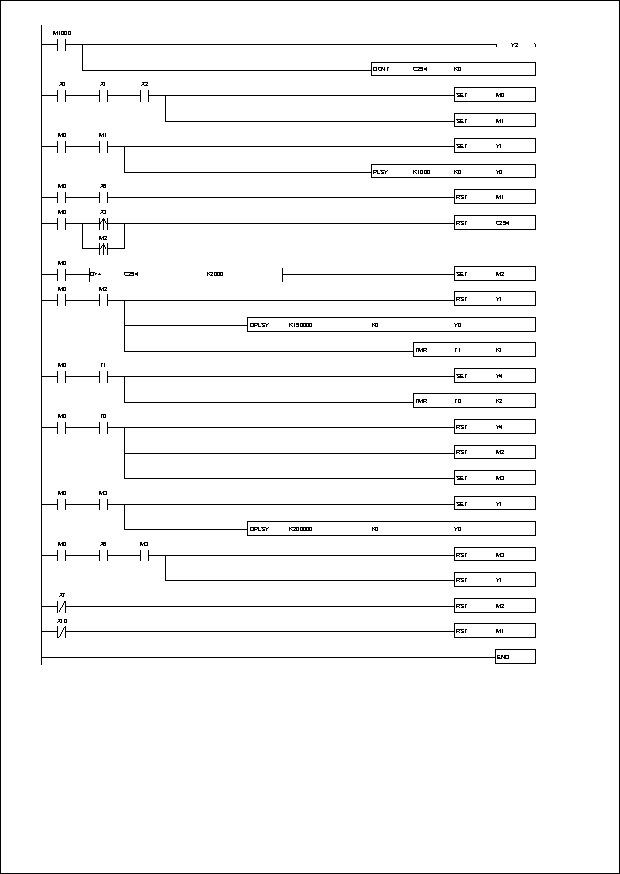
\includegraphics[width=\textwidth]{resources/code/flying_shear_code.pdf} 
    \caption[المخطط السلمي لخوارزمية المقص الطائر]{\centering المخطط السلمي لخوارزمية المقص الطائر، يوضح شبكات المزامنة، العدادات السريعة، وحماية نهايات الشوط.}
    \label{fig:ladder_code}
\end{figure}
